\part{Equazioni Differenziali}
\chapter{Equazioni Differenziali}
\section{Preliminari}
Equazione è un ugualianza in cui c'è almeno una incognita.\\
Equazione differenziale è un particolare tipo di equazione e stabilisce una relazione tra la funzione incognita e le sue derivate.In un equazione funzionale si cerca l'ugualianza di: insieme di arrivo, insieme di partenza, corrispondenza.\\
Non è necessario sapere il valore della soluzione ma sapere che ne esiste una.????????\\
Equazione differenziale ordinaria:\\
1- La funzione incognita è funzione di una sola variabile solitamente il tempo.\\
2- La funzione incognita e le sue derivate sono calcolate allo stesso istante di tempo.\\
\definition
Si dice equazione differenziale ordinaria di ordine $n$ nella funzione incognita $x\in \R^k$ un espressione del tipo:\\
$$f(t,x,\overset{\cdot}{x},\ldots,x^{(n)})=0$$
dove $f:A\to \R^m$, $A\subseteq \R^{1+(1+n)k}$ e $t\in \R$.\\
Soluzione di questa equazione differenziabile è una qualunque funzione $x:I\to \R^k$ definita su un intervallo $I\subseteq \R$, derivabile $n$ volte in $I$ e tale che $\forall t\in I$\\
$$ (t,x,\overset{\cdot}{x},\ldots,x^{(n)}) \in A$$
$$ f(t,x,\overset{\cdot}{x},\ldots,x^{(n)})=0$$
Soluzione massimale  di un equazione differenziale ordinaria è una soluzione $x_m:I_m\to \R^k$ tale che nesuna soluzione possa essere definita in un intervallo $I$ con $I_m\subseteq I_m$
\definition
un'equazione differenziale è in forma normale  se e solo se si presenta nella forma 
$$x^n = g(t,x,\overset{\cdot}{x},\ldots,x^{n-1}))$$
\observation
lo studio di unj equazione differenziale ordinaria in forma non normale inizia generalmente con l'utilizzo del Teorema della Funzione Implicita insieme ai teoremi sulle equazioni differenziali ordinarie in forma normale
\observation
illeggibile
\proposition
ogni equazione differenziale ordinaria  in forma normale di ordine $n$ è equivalente a una equazione differenziale ordinaria in forma normale di ordine $1$.\\
\begin{proof}
CASO n=2\\
abbiamo che $\overset{\cdot\cdot}{x}=f(t,x,\overset{\cdot}{x})$\\
introduco $\overset{\cdot}{X}=\begin{bmatrix}\overset{\cdot}{x}\\\overset{\cdot\cdot}{x}\end{bmatrix}$ e $X=\begin{bmatrix}x\\\overset{\cdot}{x}\end{bmatrix}$\\
quindi $\overset{\cdot}{X}=f(t,X)$
\end{proof} 
\observation
in generale un problema si dice BEN POSTO o BEN POSTO NEL SENSO DI HADAMARD ogniqualvolta:
\begin{enumerate}
	\item esisste
	\item è unica
	\item dipende con continuit\'a dai dati
\end{enumerate} 
\definition
si diche problema di Cauchy del primo ordine il problema di determinare una soluzione di un equazione differenziale ordinaria del primo ordine soddisfacente ad una condizione iniziale.\\
c'e una nota sul ben posto.......\\
$$\left\{\begin{matrix}
\overset{\cdot}{x}=f(t,x)\\x(t_0)=x_0
\end{matrix}\right.$$
Dove $f:J\times A\to \R^n$, $J\subseteq \R$ è un intervallo, $t_0\in\overset{\circ}{J}$, $A\in \R^n$, $x_0\in\overset{\circ}{A}$.\\
Soluzione di un problema di Cauchy è una funzione $x:J\to \R^n$ che sia soluzione dell'equazione differenziale $\overset{\cdot}{x}=f(t,x)$ definita in un intervallo $I$ contenente $t_0$ nella sua parte interna, $I\subseteq J$, tale che $x(t_0)=x_0$ e $x(I)\subseteq A$, e x derivaile.
\observation
la condizione $x(t_0)=x_0$ viene abitualmente chiamata condizione iniziale nonostante la definizione di soluzione richieda che la stessa sia definita in un intervallo contenente $t_0$ nella sua parte interna. In molte applicazioni delle equazioni differenziali ordinare $t_0$ è proprio l'inizio dell'intervallo in cui si cerca la soluzione. I risultati seguenti continuano a valere con piccole modifiche alle dimostrazioni.??????????
\section{La Legge di Malthus}
Una popolazione, dotata di tutto il necessario per vivere e riprodursi, cresce secondo la legge di Malthus: la velocit\'a di crescita della popolazione è proporzionale alla prpolazione stessa.\\
$$\overset{\cdot}{x}=k\cdot x$$
dove $x$ è il numero di membri della popolazione e $k$ è una costante positiva legata alla prolificit\'a della specie in esame, generalmente calcolaa come differenza tra i tassi di natalit\'a e di mortalit\'a.\\
Il problema di Cauchy è quindi $\left\{\begin{matrix}\overset{\cdot}{x}=k\cdot x\\x(0)=0\end{matrix}\right.$ con $x\in \R, k>0 $ e $ x_0=0$

\begin{center}
	\begin{tikzpicture}[scale=1] %[x={10.0pt},y={10.0pt}]
	\pgfmathsetmacro\MAX{2}
	\draw[->] (-\MAX,0) -- (\MAX,0) node[anchor=north west] {x};
	\draw[->] (0,-\MAX) -- (0,\MAX) node[anchor=south east] {$\overset{\cdot}{x}$};
	\draw[domain=-2:2,smooth,variable=\x] plot ({\x},{\x}) node {$\overset{\cdot}{x}=kx$};
	\draw node at (0.5,0) {$|$};
	\draw node at (1,0) {$|$};
	\draw node at (1.5,0) {$|$};
	\draw node at (0,0.5) {$-$};
	\draw node at (0,1) {$-$};
	\draw node at (0,1.5) {$-$};
	\draw node[anchor=north] at (0.5,0) {$x_0$};
	\draw node[anchor=north] at (1,0) {$x_0+h$};
	\draw node[anchor=north] at (1.5,0) {$x_0+2h$};
	\draw node[anchor=east] at (0,0.5) {$\overset{\cdot}{x}^{'} $};
	\draw node[anchor=east] at (0,1) {$\overset{\cdot}{x}^{''} $};
	\draw node[anchor=east] at (0,1.5) {$\overset{\cdot}{x}^{'''}$};
	
	\end{tikzpicture}% pic 1
	\qquad % <----------------- SPACE BETWEEN PICTURES
	\begin{tikzpicture}[scale=1] %[x={10.0pt},y={10.0pt}]
	\pgfmathsetmacro\MAX{2}
	\draw[->] (-\MAX,0) -- (\MAX,0) node[anchor=north west] {t};
	\draw[->] (0,-\MAX) -- (0,\MAX) node[anchor=south east] {x};
	\end{tikzpicture}% pic 2
\end{center}

blablabla ....\\
.......\\
Limiti di questo modello:
\begin{description}
	\item[-] la variabile $x$ dovrebbe variare in $N$, poich\'e una popolazione ha un numer intero di elementi.
	\item[-] In molte specie è verosimile che il numero di nati al tempo $t$ dipenda dalla popolazione presente ad un tempo precedente $x(t-T), T>0$
	\item[-] Suppore che una popolazione abbia per sempre a disposizione risorse sufficienti pu\'o non essere realistico
	\item[-] Questo modello va bene quando si considereano intervalli di tempo molto lunghi.
\end{description}

\section{Teoria Locale}
\definition Una funzione $f:I\times A\to \R^{?}$ .... $A=A\overset{\circ}{A}\subseteq \R^n$, si dice localmente lipschitziana??? .... uniformemente rispetto a $t$ se $$\forall X_0 \in A, \exists ???? : \forall x_1,x_2 \in B(x_0,r)\cap A, \forall t\in I, .......$$
\proposition
Siano $I\subseteq \R$ un intervallo aperto, .....????...., ogni funzione $f\in C^1(I,R^n)$ è localmente lipschitziana??? ..... uniformemente rispetto a $t\in I$.
\begin{proof}
	sia $x\in A \Leftarrow \exists B(x_0,r)\subseteq A$ con $r>0$, anche $\overline{B(x_0,r)}\subseteq A$ scelto $r$ abbastanza piccolo, allora $\left\| f(t,x_2)-f(t,x_1)\right\|le\sup\limits_{(t,x)\in I\times \overline{B(x_0,r)}}\left\| Df() \right\|\left\| x_2-x_1 \right\|  $ per la formula degli ccrescimenti finiti.  
\end{proof}
\subsection{Esistenza e Unicit\'a}
\proposition{Teorema di Peano}
Si consideri ilseguente problema di Cauchy: $\left\{\begin{matrix}\overset{\cdot}{x}=f(t,x)\\x(t_0)=x_0\end{matrix}\right.$ con $f:I\times A\in \R^n$ soddisfacente alle ipotesi:
\begin{enumerate}
	\item $I\subseteq \R$ intervallo, $A\subseteq \R^n, t_0\in \overset{\circ}{I}, x_0\in \overset{\circ}{A}$
	\item $f\in C^0(I\times A;R^n)$
\end{enumerate}
Allora esiste una soluzione, cio\'e $\exists J\subseteq I$ intervallo e $\exists \varphi:J\to \R^n$ con le propriet\'a:
\begin{description}
	\item[-] $J\subseteq I, \varphi(J)\subseteq A$
	\item[-] $t_0 \in \overset{\circ}{J}, \varphi(t_0)=x_0$
	\item[-] $\varphi$ derivabile e $\varphi^{'}(t)=f(t,\varphi(t))$
\end{description}
\observation 
?????????????????????????????????????????????\\
ESEMPIO Il Baffo/Pennello di Peano\\
$\left\{\begin{matrix}\overset{\cdot}{x}=\sqrt{|x|}\\x(0)=x_0\end{matrix}\right.$
\begin{center}
	\begin{tikzpicture}[scale=1] %[x={10.0pt},y={10.0pt}]
	\pgfmathsetmacro\MAX{2}
	\draw[->] (-\MAX,0) -- (\MAX,0) node[anchor=north west] {x};
	\draw[->] (0,-\MAX) -- (0,\MAX) node[anchor=south east] {$\overset{\cdot}{x}$};
	\draw[domain=0:2,smooth,variable=\x] plot ({\x},{(\x)^(1/2)});
	\draw[domain=-2:0,smooth,variable=\x] plot ({\x},{(-\x)^(1/2)});
	%\draw node at (0.5,0) {$|$};
	%\draw node at (1,0) {$|$};
	%\draw node at (1.5,0) {$|$};
	%\draw node at (0,0.5) {$-$};
	%\draw node at (0,1) {$-$};
	%\draw node at (0,1.5) {$-$};
	%\draw node[anchor=north] at (0.5,0) {$x_0$};
	%\draw node[anchor=north] at (1,0) {$x_0+h$};
	%\draw node[anchor=north] at (1.5,0) {$x_0+2h$};
	%\draw node[anchor=east] at (0,0.5) {$\overset{\cdot}{x}^{'} $};
	%\draw node[anchor=east] at (0,1) {$\overset{\cdot}{x}^{''} $};
	%\draw node[anchor=east] at (0,1.5) {$\overset{\cdot}{x}^{'''}$};
	
	\end{tikzpicture}% pic 1
	\qquad % <----------------- SPACE BETWEEN PICTURES
	\begin{tikzpicture}[scale=1] %[x={10.0pt},y={10.0pt}]
	\pgfmathsetmacro\MAX{2}
	\draw[->] (-\MAX,0) -- (\MAX,0) node[anchor=north west] {t};
	\draw[->] (0,-\MAX) -- (0,\MAX) node[anchor=south east] {x};
	\end{tikzpicture}% pic 2
\end{center}
Se $x_0 = 0$ ho che $\varphi(t)=0$ è soluzione $\forall t$\\
Ma $\overset{\cdot}{x} = \sqrt{|x|}$ è anche un'equazione a variabili separabili quindi risolvibile.\\
$$\frac{\overset{\cdot}{x}}{\sqrt{|x|}}=1 \Rightarrow \int\limits_{0}^{t}{\frac{\overset{\cdot}{x}}{\sqrt{|x|}}dt} = t$$
$$\int\limits_{x(0)=0}^{x(t)}{\frac{1}{\sqrt{|x|}}dx} = t$$
valuto ora il caso $x>=0$ quindi $|x|=x$
$$ \int\limits_{x(0)=0}^{x(t)}{\frac{1}{\sqrt{x}}dx} = 2\sqrt{x} = t$$ 
la soluzione cercata è quindi $x(t)=\frac{1}{4}t^2$, 
estendendo il ragionamento ai tempi negativi si trova che la soluzione cercata \'e: $$\varphi(x)= \left\{\begin{matrix}+\frac{1}{4}t^2&&t>0,\\0&&t=0\\-\frac{1}{4}t^2&&t<0\end{matrix}\right.$$ 
Abbiamo trovato che per la condizione iniziale $x_0=0$ il sistema ammette due soluzioni, si riesce estendere la soluzione a invinite funzioni.
$$\varphi(x)= \left\{\begin{matrix}-\frac{1}{4}(t-a)^2&&t<a,\\0&&t\in[a,b]\\+\frac{1}{4}(t-b)^2&&t>0\end{matrix}\right.$$
infatti:
$$\varphi^{'}(t) = \left\{\begin{matrix}-\frac{1}{8}(t-a)&&t<a,\\0&&t\in[a,b]\\+\frac{1}{8}(t-b)&&t>0\end{matrix}\right.$$ $$\left\{\begin{matrix}-\frac{1}{8}(t-a)=\frac{-\frac{1}{4}(t-a)^2}{	\sqrt{-\frac{1}{4}(t-a)^2}}&&t<a,\\0=0&&t\in[a,b]\\+\frac{1}{8}(t-b)=\frac{\frac{1}{4}(t-b)^2}{\sqrt{\frac{1}{4}(t-b)^2}}&&t>0\end{matrix}\right. = ....????? sistema $$
Abbiamo quindi trovato infinite soluzioni.\\
Questo esempio per sottolineare che il teorema di peano non garantisce l'unicit'a della soluzione
ESEMPIO CONTINUIT\'A è IPOTESI NECESSARIA\\
Questo esempio mostra che se non c'è continuti'\'a, pu\'o?????????? non esserci la soluzione.\\
Dato il seguente problema di Cauchy: $\left\{\begin{matrix}
\overset{\cdot}{x} = \left\{\begin{matrix}1&&x<0\\-1&&x\ge 0\end{matrix}\right.\\
x(0)=0
\end{matrix}\right.$\\
\begin{center}
	\begin{tikzpicture}[scale=1] %[x={10.0pt},y={10.0pt}]
	\pgfmathsetmacro\MAX{2}
	\draw[->] (-\MAX,0) -- (\MAX,0) node[anchor=north west] {x};
	\draw[->] (0,-\MAX) -- (0,\MAX) node[anchor=south east] {$\overset{\cdot}{x}$};
	\draw[domain=0:2,smooth,variable=\x] plot ({\x},{1});
	\draw[domain=-2:0,smooth,variable=\x] plot ({\x},{-1});
	\draw node at (0,-1) {$\bullet$};
	\draw node at (0,1) {$\circ$};
	\end{tikzpicture}% pic 1
\end{center}

$x(t)=0$ soddisfa la condizione iniziale ma ovviamente nn pu\'o essere soluzione del problema poich\'e per $x\ne 0$ si ha che $\overset{\cdot}{x}=\pm 1$ che non è la derivata della funzione nulla.\\
partendo sempre dalla condizione iniziale si pu\'o ipotizzare per esempio che la soluzione cresca, solo che questo contraddice $\overset{\cdot}{x}(0)=-1$\\
se invece si ipotizza che decresce da $0$ si ottiene che la funzione assume valori negativi, anche questo è un assurdo poich\'e la derivata per valori negativi della funzione è positiva.\\
Precisiamo che se il problema fosse stato $\left\{\begin{matrix}
\overset{\cdot}{x} = \left\{\begin{matrix}1&&x<0\\-1&&x\ge 0\end{matrix}\right.\\
x(0)=-3\end{matrix}\right.$ allora la funzione $\varphi(x)=-x+3$ sarebbe stata soluzione nell'intervallo $J=\left] -\infty,0 \right[ $
\proposition{Teorema di Cauchy Locale}
In sostanza si dimostra che il problema di Cauchy è ben posto nel senso di Hadamard.\\
Si consideri il problema di Cauchy: 
$\left\{
\begin{matrix}
\overset{\cdot}{x}=f(t,x)\\x(t_0)=x_0
\end{matrix}
\right.$\\
con $f:I\times A \to \R^n$ soddisfacente le ipotesi:
\begin{enumerate}
	\item $I\subseteq \R^n$ intervallo, $t_0\in \overset{\circ}{I}, A\subseteq \R^n, x_0\in \overset{\circ}{A}$ 
	\item $f\in C^0(I\times A; \R^n)$ queste prime due ipotesi garantiscono l'esistenza, Thm.Peano.
	\item $f$ è localmente Lipschitziana in $x\in A$ uniformemente rispetto a $t\in I$
\end{enumerate}
Allora:
\begin{enumerate}
	\item Esistenza\\
	$\exists J\subseteq I, \exists\varphi : J \to \R^n$ con le propriet\'a\\
	$\varphi soluzione:
	\left\{
	\begin{matrix}
	\ast && J\subseteq I, \varphi(J)\subseteq{A}\\
	\ast && t_o\in\overset{\circ}{J}, \varphi(t_0)=x_0\\
	\ast && \varphi derivabile, \overset{\cdot}{\varphi}(t)=f(t,\varphi(t)) \quad\forall t\in J\end{matrix}\right.$
	\item Unicit\'a\\
	Se $\exists J_1,J_2$ intervalli con $J_1\subseteq I,J_2\subseteq I$ e $\exists \varphi_1:J_1\to \R^n, \varphi_2:J_2\to \R^n$ soluzioni, cio\'e\\
	$\varphi_1,\varphi_2 soluzione:
	\left\{
	\begin{matrix}
	\ast && J_1\subseteq I,J_2\subseteq I, \varphi_1(J_1)\subseteq{A},\varphi_2(J_2)\subseteq{A}\\
	\ast && t_o\in\overset{\circ}{J_1},t_o\in\overset{\circ}{J_2} \varphi_1(t_0)=x_0, \varphi_2(t_0)=x_0\\
	\ast && \varphi_1,\varphi_2 derivabili, \overset{\cdot}{\varphi_1}(t)=f(t,\varphi_1(t)) \quad\forall t\in J_1
	\overset{\cdot}{\varphi_2}(t)=f(t,\varphi_2(t)) \quad\forall t\in J_2
	\end{matrix}\right.$
	Si pu\'o osservare che $J_1\cap J_2$ è non vuoto poic\'e entambi gli insiemi contengono $t_0$ nella loro parte interna.\\
	Allora $\forall t \in(J_1\cap J_2)$ vale $\varphi_1(t)=\varphi_2(t)$,cio\'e se esistono due soluzioni ovunque entrambe siano definite esse coincidono..\\
	\item Dipendenza Continua Dai Dati\\
	Si considerino i problemi di Cauchy che hanno la condizione iniziale nello stesso istante:
	$$ 
	(1)\left\{
	\begin{matrix}
	\overset{\cdot}{x}=f(t,x)\\x(t_0)=x_0
	\end{matrix}
	\right.\quad
	(2)\left\{
	\begin{matrix}
	\overset{\cdot}{y}=g(t,y)\\y(t_0)=y_0
	\end{matrix}
	\right.
	$$
	con $f,g:I\times A \to \R^n$ soddisfacenti le ipotesi allora esiste un $\delta >0$ tale che sull'intervallo $\left[ t_0-\delta,t_0+\delta \right]$ sono definite una soluzione $\varphi$ di (1) ed una soluzione $\psi$ di (2). Inoltre esiste $L>0$ t.c. $\forall t\in \left[t_0-\delta,t_0+\delta\right]$ vale:
	$$ 
	\left\| \varphi(t)-\psi(t) \right\| 
	\le 
	(\left\| x_0-y_0 \right\|+\delta\left\| f-g \right\|_{C^0})e^{L|t-t_0|}  
	$$
	dove $\left\| f-g \right\|_{C^0}=\sup\limits_{I\times A}\left\|f(t,x)-g(t,x)\right\|$
\end{enumerate}
\observation
L'equazione integrale 
$$x(t)=x_0+\int\limits_{t_0}^{t}f(\tau,x(\tau))d\tau$$
viene spesso denominata EQUAZIONE DI VOLTERRA.\\
Questa equazione ha senso anche per alcune funzioni $f$ non non continue ma solo misurabilinel primo argomento. Ne consegue che nei Teoremi di esistenza ed unicit\'a (locali/globali) l'ipotesi "$f$ continua" pu\'o essere sostituita da "$f$ continua tratti in $t, \forall x$, continua in $x$ e limitata"
\observation
la norma dell'integrale è minore uguale dell'integrale della norma.
\proposition LEMMA DI GRONWALL\\
Dati $a,b\in \R$ con $a\le b$ siano $\delta_0\in \left[ 0;+\infty \right]$ e $\delta,\kappa:\left[a,b\right]\to \R$ funzioni continue su $\left[a,b\right]$ con $\delta(t)\ge 0$,$\kappa(t)\ge 0 \quad \forall t\in\left[ a,b\right] $ e $\delta(t)\le \delta_0+\int\limits_{a}^{t}\kappa(\tau)\delta(\tau)d\tau$Allora $$\delta(t)\le\delta_0e^{\int\limits_a^t\kappa(\tau)d\tau}$$
Questo teorema porta da una stima implicita di $\delta$(sotto il segno di integrale) ad una stima esplicita 
\begin{proof}
	sia $\delta_0 > 0$. Sia $\Delta(t)=\delta_0+\int\limits_a^t\kappa(\tau)\delta(\tau)d\tau$.\\
	Vale per ipotesi che $\delta(t)\le\Delta(t)=\delta_0+\int\limits_a^t\kappa(\tau)\delta(\tau)d\tau$\\
	Sfruttando la derivata di $ln(\Delta(t))$ si ottiene $\frac{d}{dt}(ln(\Delta(t)))= \frac{\Delta^{'}(t)}{\Delta(t)}=\frac{\kappa(t)\delta(t)}{\Delta(t)}$, ed il termine $\frac{\delta(t)}{\Delta(t)}\le 1$, Integrando il primo e l'ultimo termine
	$$\int\limits_a^t\left( \frac{d}{dt}\left(ln(\Delta(t))\right) \right)\le\int\limits_a^t\kappa(\tau)d\tau$$
	$$ln(\Delta(t))\le ln(\delta_0)+\int\limits_a^t\kappa(\tau)d\tau$$
	$$ \Delta(t)\le\delta_0e^{\int\limits_a^t\kappa(\tau)d\tau} $$
	Da cui la tesi.
	Se $\delta_0=0$, ponendo $\Delta(t)=\epsilon+\int\limits_a^t\kappa(\tau)\delta(\tau)d\tau$ si ottiene $\delta(t)\epsilon$ ................... e il mio cervello sta bruciando
\end{proof}

\begin{proof}
	Cauchy Locale:\\
	L'idea alla base della dimostrazione è che vogliamo riuscire a trasformare il problrma di Cauchy in un problema di punto fisso.Prima di tutto serve una realazione che dal problema di Cauchy ci permetta di ottenere $x$ in funzione di qualcosa che dipenda da $x$.\\
	Integrando ambi i membridella prima equazione del problema di ottiene:
	$$\int\limits_{t_0}^t(\overset{\cdot}{x})d\tau=\int\limits_{t_0}^t(f(\tau,x(\tau)))d\tau$$
	$$x(t)=x_0+\int\limits_{t_0}^t(f(\tau,x(\tau)))d\tau$$
	$T$ è una funzione del tipo:
	$\begin{array}{rcl} T: ? & \to & ? \\ x & \to & Tx \end{array}$, con $y(t)=x_0+\int\limits_{t_0}^t(f(\tau,x(\tau)))d\tau$\\
	Abbiamo raggiunto un problem di npunto fisso ($x=Tx$). Ora bisogna determinare l'insieme di partenza e l'insieme di arrivo in maniera utile per la dimostrzione. Per poter applicare il Teorema delle contrazioni serve che nlo spazio di partenza e di arrivo siano uguali e chiamiamo $\mathcal{X}$.\\
	$\begin{array}{rcl} T: \mathcal{X} & \to & \mathcal{X} \end{array}$ t.c.: $y(t)=(Tx)(t)=x_0+\int\limits_{t_0}^t(f(\tau,x(\tau)))d\tau$
	Bisogna quindi scegliere l'insieme $\mathcal{X}$. è un insieme di funzioni, in cui l'equivalenza sopra deve avere senso, cio\'e serve $x$ continua per avere l'equivalenza con il problema di Cauchy, quindi $\mathcal{X}=C^0(\ldots)$.\\
	Inoltre volendo una soluzione del problema di Cauchy, la funzione $x(penso sia y(t)=x)$ deve essere definita almeno su un intervallo contenente $t_0$ nella sua parte interna, non interessa l'estensione di tale intevallo quindi si pu\'o scegliere $\left[t_0-\delta,t_0+\delta\right]$, inoltre deve avere valori in un insieme con $x_0$ nella sua parte interna, $\overline{B(x_0,r)}$. Quindi $\mathcal{X}=C^0(\left[t_0-\delta,t_0+\delta\right];\overline{B(x_0,r)})$\\
	Per $\delta, r$ abbastanza piccoli si ha $\left[t_0-\delta,t_0+\delta\right]\subseteq I$, $\overline{B(x_0,r)}\subseteq A$, quindi adesso il problema è quello di determinare $\delta, r$.\\
	Per poter applicare il teorema delle contrazioni:
	\begin{description}
		\item[a-] $Tx$ definita (possibilit\'a di calcolarla)
		\item[b-] $Tx\in\mathcal{X}$ (insiemi di partenza e arrivo)
		\item[c-] $Tx$ contrazione
		\item[d-] $\mathcal{X}$ completo
	\end{description}
	Se tutti questi punti sono soddisfatti, si pu\'o trovare $x=Tx$, cio\'e una $x$ che soddisfa l'equazione integrale e di conseguenza, per equivalenza, soluzione del problema di Cauchy.  
	\begin{description}
		\item[a-] $Tx$ definita significa poter calcolare l'integrale,per poter calcolare l'integrale devo poter calcolare la $f$, per calcolare la $f$ ho bisogno che $\tau$ e $x(\tau)$ stiano dentro gli insiemi su cui è definita la $f$, cio\'e $I,A$, per essere sicuri di non uscire dall'intervallo:
		$$\delta>0\quad t.c:\quad \left[t_0-\delta,t_0+\delta\right]\subseteq I$$
		OSS:: Se si cambiano $\delta, r$ con valori minori tutto vale ancora.\\
		OSS:: Per il problema x derivabile -> integrale  ... mi sosto in $C^0$
		\item[b-] $Tx$ deve appartenere a $\mathcal{X}$. L'insieme $\mathcal{X}$ sostanzialmente pone tre vincoli a $Tx$: deve essere $C^0$, definita in $\left[t_o-\delta;t_0+\delta\right]$ a valori in $\overline{B(x_0,r)}$.\\
		Per iniziare si verifica che sia definita in $\left[t_o-\delta;t_0+\delta\right]$\\
		.... qualchosa che non comprendo.... $C^0$\\
		Resta da verificare che $Tx$ è a valori nella sfera, cio\'e che 
		$$(Tx)(t) \in \overline{B(x_0,r)}$$
		Valuto la distanza tra $(Tx)(t)$ e $x_0$. La differenza tra la posizione al tempo $t$ e al tempo $t_0$, questa distanza pu'\o essere controllata con la velocit\'a e il tempo per cui il punto dsi è mosso.\\
		Chiamata $V$ la massima velocit\'a alla quale pu\'o muoversi il punto, $V=\sup\limits{(t_0\times X_0)\in (\left[to+\delta,t_0-\delta\right]\times\overline{B(x_0,r)})}=\left\{\left\|f(t,x(t))\right\|\right\}$ che è il sup della norma di f, cio\'e dei moduli dei vettori velocit\'a, questo esiste sempre finito, non $\infty$ poich\'e $f$ è continua, la norma è continua , $t$ varia in un chiuso e limitato, $x_0$ varia in un chiuso e limitato, quindi stiamo calcolando  il sup di una funzione continua su un chiuso e limitato allora per il teorema di Weierstrass $V=\max\limits{(t_0\times X_0)\in (\left[to+\delta,t_0-\delta\right]\times\overline{B(x_0,r)})}=\left\{\left\|f(t,x(t))\right\|\right\}$\\
		Non potendo modificare $V, \delta$ poniamo una restrizione su $r$:$V\delta < r$, da cui $\delta < r\cdot V$
		
		$$\left\|(Tx)(t) - x_0 \right\| = \left\| \int_{t_0}^t(f(\tau,x(\tau)))d\tau \right\| \le \left|\int_{t_0}^t \left\| f(\tau,x(\tau)) \right\|d\tau \right|\le$$
		$$\le\left| \int_{t_0}^t V\cdot d\tau\right|=V\left| t-t_0\right|\le V\delta<r$$
		....aggiunto il modulo per $t<t_0$ e $t>t_0$ non lo si sa a priori\\
		quidi $\left\|(Tx)(t) - x_0 \right\|$ è minore di $r$ scelto $\delta$ opportunamente piccolo. 
		\item[c-] Se $Tx$ è una contrazione deve valere che
		$$\left\| Tx_2 - Tx_1\right\|_{C^0}\le K\left\|x_2-x_1\right\|_{C^0}\quad k\in\left[0,1\right[\quad\forall t\in\left[t_0-\delta,t_0+\delta\right]$$
		con $\left\|Tx_2-Tx_1\right\|_{c^0}=\sup\limits_{t\in\left[t_0-\delta,t_0+\delta\right]}\left\| (Tx_2)(t) - (Tx_1)(t)\right\|$, partendo da questa utilizzando prima la definizione di $f$ poi la linearit\'a dell'integrale ....lipsh f... propriet\'a
		$$\left\| (Tx_2)(t) - (Tx_1)(t)\right\|=$$
		$$\left\| x_0+\int_{t_0}^t f(\tau,x_2(\tau)) d\tau - \left(x_0+\int_{t_0}^t f(\tau,x_1(\tau)) d\tau\right) \right\|=$$
		$$\left\| \int_{t_0}^t f(\tau,x_2(\tau))-f(\tau,x_1(\tau)) d\tau \right\|\le$$
		$$\left| \int_{t_0}^t \left\|f(\tau,x_2(\tau))-f(\tau,x_1(\tau))\right\| d\tau \right|\le$$
		$$\left| \int_{t_0}^t L\left\|x_2(\tau)-x_1(\tau)\right\| d\tau \right|\le$$
		$$L\left| \int_{t_0}^t \left\|x_2-x_1\right\|_{C^0(\left[t_0-\delta,t_0+\delta\right];R^n)} d\tau \right|=$$
		$$L\cdot \left\| x_2-x_1 \right\|_{C^0(\left[t_0-\delta,t_0+\delta\right];R^n)}\left|t-t_0\right|\le$$
		$$L\delta\left\|x-x_0\right\|_{C^0(\left[t_0-\delta,t_0+\delta\right];R^n)}$$
		cio\'e $\forall t \in \left[t_0-\delta,t_0+\delta\right]$ vale che $\left\|(Tx_2)(t)-(Tx_1)(t)\right\|\le L\delta\left\|x_1-x_2\right\|_{C^0(\left[t_0-\delta,t_0+\delta\right];R^n)}$ e poiche è vero $\forall t \Rightarrow $ passando all'estremo superiore
		$$ \left\| Tx_1 - Tx_2 \right\|_{C^0(\left[t_0-\delta,t_0+\delta\right];R^n)}\le L\delta\left\|x_1-x_2\right\|_{C^0(\left[t_0-\delta,t_0+\delta\right];R^n)}$$
		A questo punto scelto $\delta$ t.c. $L\delta<1$ ad esempio $\delta=\frac{1}{2L}$ cos\'i ottengo che per $\delta$ opportuno $Tx$ è una contrazione.		
		\item[d-] Bisogna mostrare che $\mathcal{X}$ è completo.\\
		Supponiamo che $\mathcal{X}\subseteq C^0(\left[t_0-\delta,t_0+\delta\right];R^n)$, questo insieme è completo rispetto alla metrica $d_\infty=d_{C^0}$, allora se abbiamo una successione $x_n$ di Cauchy in $\mathcal{X}$ lo è anche su $C^0(\left[t_0-\delta,t_0+\delta\right];R^n)$, allora $\exists x_\infty\in C^0(\left[t_0-\delta,t_0+\delta\right];R^n)$ con $x_n\to x_\infty$ per $n\to\infty$, ma poich\'e $\forall t \in\left[t_0-\delta,to+\delta\right]$ $x_\infty(t)=\lim\limits_{n\to\infty}x_n(t)$ e visto che $\forall t,\forall n\quad \left\| x_n(t)-x_0\right\|\le r$ anche al limite vale $\left\| x_{\infty}(t)-x_0\right\|\le r \Rightarrow x_\infty\in\mathcal{X}$ cio\'e $\mathcal{X}$ è completo.
	\end{description}
	Possimao a questo punto applicare il teorema delle Contrazioni allora $T$ ha un unico punto fisso allora l'equazione integrale ha un unica soluzione allora esiste la soluzione del problema di Cauchy e su $\left[t_0-\delta,t_0+\delta\right]$ possiamo gia dire che la soluzione  è unica.\\
	MA QUANTO CAZZO è LUNGA FORSE SONO A MET\'A\\
	\begin{center}
		\begin{tikzpicture}[scale=2]
		\draw[->] (-0.5,0) -- (2,0) node[anchor=north west] {$t$};
		\draw[->] (0,-0.5) -- (0,2) node[anchor=south east] {$x$};
		%\draw[domain=0:2,smooth,variable=\x] plot ({\x},{1});
		%\draw[domain=-2:0,smooth,variable=\x] plot ({\x},{-1});
		\draw node at (0.5,0) {$\bullet$};
		\draw node[anchor=north] at (0.5,0) {$t_0-\delta$};
		\draw node at (1,0) {$\bullet$};
		\draw node[anchor=north] at (1,0) {$t_0+\delta$};
		\draw node at (1.5,0) {$\bullet$};
		\draw node[anchor=north] at (1.5,0) {$t_0$};
		%\draw node at (0,1) {$\circ$};
		\end{tikzpicture}% pic 1
	\end{center}
	FINIRE DISEGNO......\\
	OSS:: Passando da (a-), (d-) abbiamo ristretto sempre pi\'u il range di valori che $\delta, r$ possono assumere, cos\'i che alla fine è rimasto un intervallo sul quale è applicabile il teorema delle Contrazioni.\\
	Abbiamo trovato un intervallo $\left[t_0-\delta,t_0+\delta\right]$ in cui la soluzione esiste. Adesso osserviamo cosa accade prima a destra e poi a sinitra dell'intervallo con un ragionamento analogo.\\
	Soluzioni che sono coincidenti(cio\'e unica) in un intervallo possono non esserlo al difuori dello stesso. Cauchy locale ci assicura che questo non pu\'o succedere.\\
	Sia per assurdo $t_M$ l'ultimo istante fino a cui $\varphi_1,\varphi_2$ coincidono, cio\'e: $t_M = \sup \left\{t\in I:t\ge t_0, \varphi_1(\tau)=\varphi_2(\tau), \forall \tau \in \left[t_0,t\right[\right\}$.\\
	Cerchiamo di mostrare o che non c\'e o che è alla fine dell'intervallo $I$.\\
	Sesi considera il problema di Cauchy:
	$\left\{\begin{matrix}\overset{\cdot}{x}=f(t,x(t))\\x(t_M)=x_{t_M}\end{matrix}\right.$. Possiamo applicare quanto trovato per il punto uno della tesi, cio\'e esiste un intervallo contenente $t_M$ nella sua parte interna in cui la soluzione esiste ed è unica.\\
	OSS:: $t_M$ esiste sempre poich\'e è il $sup$ di un insieme non vuoto, inoltre $t_M\ge t_0+\delta$ è certamente $t_M\in \overline{I}$\\
	Possono verificarsi due casi, o $t_M$ è sul bordo di $I$ ed in questo caso la dimostrazione è finita poich\'e fino al bordo dell'intervallo le soluzioni coincidono.
	Oppure $T_M$ è nella parte interna dell'intervallo quindi $t_m\ne\sup I\Rightarrow t_M\in\overset{\circ}{I}$, e se è u n punto interno per l'intervallo allora è anche un punto di accumulazione per lo stesso, è quindi possibile calcolare $\lim\limits_{t\to t_M^{-}}\varphi_1(t)\quad\lim\limits_{t\to t_M^{-}}\varphi_2(t)$ ma entrambi i limiti devono essere uguali a $x_M$ poich\'e sia $\varphi_1,\varphi_2$ sono soluzioni al problema  di Cauchy e devono quindi soddisfare la condizione iniziale, anche perché fino a $t_M$ le due soluzioni coincidono e quindi il loro limite deve essere lo stesso.\\
	Riguardo $x_M$ si pu\'o dire che:
	\begin{enumerate}
		\item se $x_M = A\Rightarrow$ le soluzioni coincidono fino alla fine dell'insieme $A$.
		\item se $x_m\in\overset{\circ}{A}$ abbiamo esattamente le ipotesi del teorema di Cauchy locale, per quanto visto si ha necessariamente che:\\
		$\exists \delta_M>0,\exists \varphi_M:\left[t_M-\delta_M,t_0+\delta_M\right]\to \R^n$ che è soluzione del nuovo problema impostato, UNICA per quanto detto sull'intevallo.
	\end{enumerate} 
	Applicando il ragionamento funo a quando non si raggiungono i bordi di $I$ e di $A$ abbiamo dimostrato che se esistono pi'\u soluzioni allora queste coincidono dove sono definite entrambe.\\
	FATTO IL SECONDO PUNTO DEL TEOREMA.\\
	Dati
	$$(P_f):\left\{\begin{matrix}\overset{\cdot}{x}=f(t,x(t))\\x(t_0)=x_{0}\end{matrix}\right.\quad	(P_g):\left\{\begin{matrix}\overset{\cdot}{y}=f(g,y(t))\\y(t_0)=y_{0}\end{matrix}\right.$$
	Siano $\varphi$ soluzionedi $P_f$, $\psi$ soluzione di $P_g$, bisogna stimare quanto queste due soluzioni di due problemi con la condizione iniziale allo stesso istante distano.
	$$\varphi:\left[t_0-\delta_f,t_0+\delta_f\right]\to \R^n$$
	$$\psi:\left[t_0-\delta_g,t_0+\delta_g\right]\to \R^n$$
	chiamo $\delta=\min{\delta_f,\delta_g}$ che sicuramente soddisfa entrambe. Per stimare la distanza tra le soluzioni valuto:
	$$
	\left\|\varphi(t)-\psi(t)\right\|=
	\left\|  x_0+\int_{t_0}^t f(\tau,\varphi(\tau))d\tau - y_0 - \int_{t_0}^t g(\tau,\psi(\tau))d\tau\right\|
	$$
	linearit\'a integrale disugualianza norama... modulo per i differenziali ....\\
	$$ \left\| x_0-y_0\right\|+\left| \int_{t_0}^{t} \left\| f(\tau,\varphi(\tau))-g(\tau,\psi(\tau)) \right\|d\tau \right|\le$$
	adesso all'interno dell'integrale aggiungo e tolgo la quantit\'a $f(\tau,\psi(\tau))$ e applico la disugualianza triangolare riarrangiando i termini
	$$ \left\| x_0-y_0\right\|+\left| \int_{t_0}^{t} \left\| f(\tau,\varphi(\tau))-f(\tau,\psi(\tau))\right\|+\left\|f(\tau,\psi(\tau))-g(\tau,\psi(\tau)) \right\|d\tau \right|\le$$
	$$ \left\| x_0-y_0\right\| + \left\| f-g\right\|_{c^0}\left|t-t_0\right| +\left| \int_{t_0}^{t} L\left\|\varphi(\tau)-\psi(\tau)\right\| d\tau \right|$$
	per comodit\'a restringiamo la trattazione al caso $t>t_0$ sparisce il modulo. Rscrivo il primo e l'ultimo membro della disugualianza
	$$ \left\|\varphi(t)-\psi(t)\right\|\le  \left[ \left\| x_0-y_0\right\| + \delta\left\| f-g\right\|_{c^0}\right] +\left| \int_{t_0}^{t} L\left\|\varphi(\tau)-\psi(\tau)\right\| d\tau \right|$$
	$$ \left( \delta(t)\le\delta_0+\int_{t_0}^t \kappa(\tau)\delta(\tau)d\tau \right)::Gronwall$$
	$$ \left\| \varphi(t)-\psi(t)\right\|\le\left[\left\|x_0-y_0\right\|+\delta\left\|f-g\right\|_{C^0}\right]+e^{L\left|t-t_0\right|}$$
	QUESTO TEOREMA è TROPPO DA PRO.
\end{proof}
ESEMPIO: DECADIMENTO RADIOATTIVO\\
Il decadimento di una sostanza radioattiva è ben descritto da $\overset{\cdot}{x}=-k\cdot x$ dove $x$ è la quantit\'a di sostanza radioattiva non ancora decaduta e $k$ è una costante propria di ogni singolo materiale\\
...........\\
ESEMPIO: LEGGE DEL CALORE DI NEWTON\\
......\\
ESEMPIO: CRESCITA LOGISTICA\\
......\\
\section{Teoria Globale}
\proposition
Siano $(X,d_x)$ e $(Y,d_y)$ spazi metrici, sia $f:A\subseteq X\to Y$. Se $f$ è uniformemente continua su $A$ allora $\exists ! \overline{f}:\overline{A}\to Y$ t.c. $\overline{f}_{\left|A\right.}=f$. Cio\'e $f$ pu\'o essere estesa in modo unico alla chiusura dell'insieme $A$.
\definition
Una funzione $f:I\times \R^n\to \R^n$ con $I$ intervallo in $R$ si dice sub lineare se esistonop due costanti posirive $A$ e $B$ t.c.: $\forall t \in I$ 
$$ \left\| f(t,x) \right\|\le A + B\left\|x\right\|$$\\
ESEMPIO:: $f(t,x)=x^2$ NON SUBLINEARE\\
ESEMPIO:: $f(t,x)=sin(x^2)$ SUBLINEARE\\
\observation 
Sia $f(t,x)$ globalmente Lipshitziana in $x$ uniformemente in $t$ allora $f$ sublineare.
$$\exists L\ge 0 :\forall x_1,x_2\in \R^n, t\in I, \left\|f(t,0)\right\|\le A$$
$$\left\| f(t,x_2)-f(t,x_1) \right\|\le\left\|x_2-x_1\right\|$$
$$\left\| f(t,x)\right\|\le\left\|f(t,x_0)\right\|+\left\|f(t,x)-f(t,0)\right\|\le A +L\left\|x\right\|$$
In sostanza una funzione è sublineare se esiste una retta tale per cui il grafico della funzione è tutto nella regione di piano delimitata da questa retta.
	\begin{center}
	\begin{tikzpicture}[scale=2]
	\draw[->] (-2,0) -- (2,0) node[anchor=north west] {$x$};
	\draw[->] (0,-2) -- (0,2) node[anchor=south east] {$y$};
	\draw[domain=-2:2,smooth,variable=\x] plot ({\x},{0.25*abs(\x)+0.5});
	\draw[domain=-2:2,smooth,variable=\x] plot ({\x},{-(0.25*abs(\x)+0.5)});
	\end{tikzpicture}% pic 1
\end{center}
ESEMPIO::$x\cdot sin(x)$ SUBLINEARE\\
ESEMPIO::$x^2\cdot sin(x)$ NO SUBLINEARE\\
ESEMPIO::$e^x$ NO SUBLINEARE\\
Diciamo sublineare se il grafico nn si impenna.\\
\proposition
Data la funzione $f:I\times \R^n\to \R^n$, se:
\begin{enumerate}
	\item $I\subseteq \R$ è un intervallo, con $t_0\in\overset{\circ}{R^n}$
	\item $f\in C^0(I\times \R^n;R^n)$
	\item $f$ è localmente Lipschitziana in $x\in \R^n$ uniformemnte rispetto $t\in I$
	\item $f$ è sublineare
\end{enumerate}
allora il problema di Cauchy $\left\{\begin{matrix}\overset{\cdot}{x}=f(t,x)\\x(t_0)=x_0\end{matrix}\right.$ ammette un'unica soluzione definita sull'intervallo $I$.
\begin{proof}
	DISEGNO...\\
	Il teorema di Cauchy Locale assicura che  la soluzione esiste unica su un intervallo centrato all'istante iniziale.
	Bisogna dimostrazre che la soluzioe pu\'o essere estesa a tutto l'intervallo. Questo nn si pu\'o fare in due casi:
	\begin{enumerate}
		\item c'è un asintoto verticale
		\item oscilla tanto che a un certo punto non va pi\'u avanti
	\end{enumerate}
	Quindi i casi in cui la soluzione non si pu\'o estendere su tutto l'intervallo sono quelli in cui non esiste il limite della soluzione. Quindi dobbiamo evitare tali comportamenti.\\
	Ragionamento da $t_0$ in avanti.\\
	Sia $T=sum\left\{t\in I :\exists soluzione su \left[ t_0,t \right[ \right\}$ cio\'e prendo l'estremo superiore dei tempi per cui c'è una soluzione.
	Se $T= sup I$ o $T=+\infty$ abbiamo la tesi.\\
	Se $T$ finito con $T<sup I$, dimostrando che la derivata della soluzione è limitata si escludono i casi in cui l'estensione della soluzione non si pu\'o fare.
	quindi bisogna mostrare $\overset{\cdot}{x} = f(t,x)$ è limitata sull'insieme dove pu\'o arrivare la $x$\\
	Sia ora $\varphi$ soluzione del problema di Cauchy:
	$$ \varphi(t) = x_0 + \int_{t_0}^tf(\tau,x(\tau))d\tau$$
	Valuto allora\\
	$\left\|\varphi(t)\right\|\le \left\|x_0\right\| + \left|\int_{t_0}^tf(\tau,\varphi(\tau))d\tau\right|=\left\|x_0\right\| + \int_{t_0}^t\left\|f(\tau,\varphi(\tau))\right\|d\tau$ poich\'e $t\in\left[t_0,T\right[$\\
	$\left\|\varphi(t)\right\|\le \left\|x_0\right\| + \int_{t_0}^t\left(A+B\left\|\varphi(\tau)\right\|\right)d\tau$ poich\'e f è sublineare.\\
	$\left\|\varphi(t)\right\|\le \left\|x_0\right\| + A(T-t_0)+\int_{t_0}^t B\left\|\varphi(\tau)\right\|d\tau$\\
	...\\
	applico ilGronwall e risulta che
	$$\left\|\varphi(t)\right\|\le\left(\left\|x_0\right\|+A(t-t_0)\right)e^{B(t-t_0)}\le\left(\left\|x_0\right\|+A(t-t_0)\right)e^{B(T-t_0)}$$	
	Abbiamo quindi dimostrato che la $f$ resta limitata.\\
	Posso guardare alla funzione come segue:\\
	$$
	\sup
	\left\{f(t,x): t\in\left[t_0,T\right[, x\in \overline{B\left(x_0,
		\left[ 
			\left\|x_0\right\| A \left(T-t_0\right)
		\right]e^{B\left(T-t_0\right)}\right)}
	\right\}
	$$
	$\overline{B\left(x_0,
		\left[ 
		\left\|x_0\right\| A \left(T-t_0\right)
		\right]e^{B\left(T-t_0\right)}\right)}
	$ è un insieme compatto poich\'e chiuso e limitato in $R^n$, $\varphi$ è limitata, la $f$ limitata, allora $\overset{\cdot}{\varphi}$ limitata allora $\varphi$ lipshitziana allora $\varphi$ uniformemente continua.\\
		Allora esiste finito $\lim\limits_{t\to T^{-}}\varphi(t)=X$. Ora possono verificarsi due casi:\\
	\begin{enumerate}
		\item Se $T=\sup I \Rightarrow$ dimostrazione conclusa
		\item Se $T<\sup I \Rightarrow$ posso considerare il problema di Cauchy \\
		$\left\{ \begin{matrix} \overset{\cdot}{x}=f(t,x)\\x(T)=X \end{matrix} \right.$ Questo è un assurdo poich\'e arriveremmo a trovare una soluzione definita oltre il tempo $T$. Questo nega la scelta fatta a inizio dimostrazione.
		\end{enumerate}
\end{proof}
\section{Equazioni Autonome}
\definition 
Un'equazione differenziale ordinaria in forma normale si dice autonoma sse la variabile indipendente (solitamente il tempo) non vi compare escplicitamente.
\observation
Tipicamente, le euqazioni differenziali ordinarie autonome modellizzano sistemi isolati.
\observation Invarianza per traslazione temporale.\\
Non è importante ai fini dello studio dell'equazione l'istante iniziale, ma solo la lunghezza dell'intervallo.
Se  $x=\varphi(t)$ risolve $\left\{ \begin{matrix} \overset{\cdot}{x} = f(x)\\x(t_0)=x_0 \end{matrix} \right.$\\
Allora $x=\varphi(t+t_0)$ risolve $\left\{ \begin{matrix} \overset{\cdot}{x} = f(x)\\x(0)=x_0 \end{matrix} \right.$\\
\begin{proof}
	Sia $\psi(t)=\varphi(t_0+t)$\\
	$\overset{\cdot}{\psi}(t)=\overset{\cdot}{\phi}(t_0+t)=f(\varphi(t_0+t))=f(\psi(t))$\\
	$\psi(0)=\varphi(t_0)=x_0$ 
\end{proof}
\proposition Teorema dell'eneria cinetica\\
Un punto materiale non vincolato $P$ di massa $m$ si muove sotto l'azione di una forza $F$ che dipende solo dalla posizione di $P$. Allora la variazione di energia cinetica di $P$ è uguale al lavoro compiuto su $P$ da questa forza.
\begin{proof}
	sia $\underline{x}=(x,y,z)$ la terna delle coordinate di $P$. Per il Secondo Principio della Dinamica e per quanto assunto sulla forza $F$, il moto di $P$ è descritto dall'equazione(vettoriale) differenziale ordinaria del secondo ordine:\\
	$$m\overset{\cdot\cdot}{\underline{x}}=F(\underline{x})$$
	$$m\overset{\cdot\cdot}{\underline{x}}\overset{\cdot}\cdot{\underline{x}}=F(\underline{x})\overset{\cdot}{\underline{x}}$$
	$$\frac{1}{2}m\frac{d}{dt}\left(\left(\overset{\cdot}{\underline{x}}\right)^2\right)=F(\underline{x})\overset{\cdot}{\underline{x}}$$
	$$\int_{0}^t\frac{1}{2}m\frac{d}{dt}\left(\left(\overset{\cdot}{\underline{x}}(\tau)\right)^2\right)d\tau=\int_{0}^tF(\underline{x}(\tau))\cdot\overset{\cdot}{\underline{x}(\tau)}d\tau$$
	$$\frac{1}{2}m\left(\overset{\cdot}{x}(t)\right)^2-\frac{1}{2}m\left(\overset{\cdot}{x}(0)\right)^2 = \int_{x(0)}^{x(t)}F(\xi)d\xi$$
	L'ultimo integrale è calcolato lungo la traiettoria di $P$.
\end{proof}
ESEMPIO:: Il Lancio di un Paracadutista\\
.....\\
.....\\
.....\\
ESEMPIO:: CADUTA IN UN LIQUIDO\\
.....\\
.....\\
.....\\
\section{Equazioni Differenziali Ordinarie}
\definition
Sia $I\subseteq\mathbb{R}$ un intervallo e $n\in N$. Date le $n+1$ funzioni $a_0,a_1,\ldots,a_{n-1}, f:I\to\mathbb{C}$ si dice equazione differenziale ordinaria lineare di ordine $n$, l'equazione differenziale:
$$x^{(n)}+a_{n-1}(t)\cdot x^{(n-1)}+\ldots+a_1(t)\cdot\overset{\cdot}{x}+a_0(t)x=f(t)$$
Se $f\equiv 0 $ l'equazione si dice omogenea.
\proposition
sia $I$ un intervallo compatto e tale che $\overset{\circ}{I}\ne \emptyset$ siano $a_0,a_1,\ldots,a_{n-1},f\in C^0(I;\mathbb{C})$. Allora $\forall t_0\in\overset{\circ}{I}$ e $c_0,c_1,\ldots,c_{n-1}\in\mathbb{C}$ il problema di Cauchy 
$$ \left\{\begin{matrix}[]
x^{(n)}=-\sum\limits_{k=1}^{n-1}\left(a_k(t)x^k\right)+f(t)\\
x(t_0)=c_0\\
x(t_2)=c_1\\
\ldots\\
x^{(n-1)}(t_0)=c_{n-1}\\
\end{matrix}\right.$$
ammette soluzine unica definita su tutto l'intervallo $I$.
\begin{proof}
	Un'equazione differenziale lineare di ordine $n$ pu\'o essere trasfprmato in un sistema di equazioni al primo ordine.
	Introduciamo la variabile $X\in\mathbb{C^n}$ ed il dato iniziale $C\in\mathbb{C^n}$
	$$\left[\begin{matrix} X_1\\X_2\\\ldots\\X_{n-1}\\X_n \end{matrix}\right] = \left[\begin{matrix} x\\\overset{\cdot}{x}\\\ldots\\ x^{(n-1)}\\x^{(n)} \end{matrix}\right]\quad\quad\left[\begin{matrix} C_1\\C_2\\\ldots\\C_{n-1}\\C_{n} \end{matrix}\right] = \left[\begin{matrix} c_0\\c_1\\\ldots\\ c_{n-2}\\c_{n-1} \end{matrix}\right]$$
	il problrma di Cauchy per l'equazione lineare diventa:
	$$
	\left\{
	\left[\begin{matrix} X_1^{'}\\X_2^{'}\\\ldots\\X_{n-1}^{'}\\X_n^{'} \end{matrix}\right]
	=
	\left[\begin{matrix} X_2\\X_3\\\ldots\\X_{n}\\-\sum\limits_{k=1}^{n-1}\left(a_k(t)x^k\right)+f(t) \end{matrix}\right]
	\\
	X(t_0)=C
	\right.
	$$
	La funzione
	$\begin{array}{rcl} 
	F: I\times\mathbb{C}^n & \to & \mathbb{C}^n \\
	   (t,X) & \to & \left[\begin{matrix} X_2\\X_3\\\ldots\\X_{n}\\-\sum\limits_{k=1}^{n-1}\left(a_k(t)x^k\right)+f(t) \end{matrix}\right] \\ 
	\end{array}$
	\'e linear in $X$ e globalmente lipshitziana in $X$ uniformemente in $t$, infatti perogni $X,Y\in\mathbb{C}^n$
	$$\left\|F(t,X)-F(t,Y)\right\|\le \sqrt{1+\left( \max\limits_k \sup\limits_I \left\|a_k\right\| \right)^2}\cdot\left\|X-Y\right\|$$
	Sono soddisfatte le ipotesi di Cauchy Globale allora si ha latesi.
\end{proof}
\observation
La locuzione lineare è giustificata dalla proposizione seguente.
\proposition
Sia $I\subseteq \R$ un intervallo e $n\in\mathbb{N}$. Date le $n+1$ funzioni $a_0,a_1,\ldots,a_{n-1},f:I\to\mathbb{C}$,l'operatore 
$\begin{array}{rcl} 
L: C^n(I;\mathbb{C}) & \to & C^0(I;\mathbb{C}) \\
x & \to & x^{(n)}+\sum\limits_{k=1}^{n-1}a_k(t)x^{(k)} \\ 
\end{array}$\'e lineare
\begin{proof}
	La linearit\'a di $L$ equivale a:
	$$ \begin{matrix}L(x_1+x_2)=L(x_1)+L(x_2) && \forall x_1,x_2\in C^n(I;\mathbb{C})\\L(\lambda\cdot x)=\lambda\cdot L(x) && \forall\lambda\in\mathbb{C}, \forall x\in C^n(I;\mathbb{C})\end{matrix} $$
	Entrambe le condizioni  seguono dalle regole di derivazione.
\end{proof}
\section{Equazioni Lineari a Coefficienti Costanti}
\definition
Dati i coefficienti $a_0,a_1,\ldots,a_{n-1},b\in\mathbb{C}$, si dice equazione differenziale ordinaria lineare di ordine $n$ a coefficienti costanti l'equazione differenziale
$$x^{(n)}+a_{n-1}x^{(n-1)}+\ldots+a_1\overset{\cdot}{x}+a_0x=b$$
se $b=0$ l'equazione si dice omogenea. La sua Equazione caratteristica è l'equazione algebrica
$$\lambda^n+a_{n-1}\lambda^{n+1}+\ldots+a_1\lambda+a_0=0$$ 
\observation
Nella risoluzione di eqauzioni differenziali lineari la funzione esponenziale $t\to e^{\lambda t}$ riveste un ruolo molto particolare. Questa funzione è un autovalore dell'operatore di derivazione $D$ relativo all'autovalore, risolve infatti $\lambda$:$Dx=\lambda\cdot x$ 
\proposition
Data l'equazione
$$x^{(n)}+a_{n-1}x^{(n-1)}+\ldots+a_1\overset{\cdot}{x}+a_0x=b$$
$x(t)=e^{\lambda t}$ risolve l'equazione omogenea $\Leftrightarrow$ $\lambda$ è soluzione dell'equazione caratteristica.\\

LEMMA:: Sia $x(t)=t\cdot e^{\lambda\cdot t}$. Allora , per ogni $n\in\mathbb{N}, n\ge 1$
$$x^{(n)}(t)=\left(\lambda^nt+n\lambda^{n-1}\right)e^{\lambda t}$$
???????????????NON L?HO CAPITA BENE.......................\\
\proposition
Data l'equazione 
$$x^{(n)}+a_{n-1}x^{(n-1)}+\ldots+a_1\overset{\cdot}{x}+a_0x=b$$
$x(t)=te^{\lambda t}$ risolve l'eqauzione omogenea $\Leftrightarrow$ $\lambda$ è soluzione dell'equazione caratteristica con molteplicit\'a almeno ??????????.






